


\begin{frame}{\citetitle{MarcoNuno_CongArbIng_2015_02_00} \footnotemark (1)}
\begin{block}{Problem description  (1)} 
\begin{itemize}

%\note[item]{\scriptsize Due to user acceptability, smartphones are able to measure nonintrusively proprioceptive motion outside of a controlled environment for rather long periods of time using embedded inertial sensors.}
\item Knowledge of human activities and behaviors are good indicators to assess human health status associated to sedentarism.
\note[item]{\scriptsize Activity recognition is a low-level enabler of mobile health (mHealth) systems}
\item Mobile health (mHealth) systems improves human health and well-being by
continuously monitoring their status.
%\note[item]{\scriptsize mHealt systems allows rapidly diagnosing, recognizing behaviors and delivering just-in-time interventions in the mobile user environment}
\item Measure nonintrusively proprioceptive motion outside of a controlled
environment is useful in several applications.
%\note[item]{\scriptsize Due to their communication, computation and sensing capabilities, smartphones have become everyday devices that many people carry with them all day long, which facilitate both remote acquisition and on-device processing of personal, social or environmental data, captured through embedded physical sensors}
\item We propose a position-independent activity recognition system for continuous real-time monitoring to be used as standalone in a smartphone.
\end{itemize}
\end{block}
\footnotetext[1]{\fullcite{MarcoNuno_CongArbIng_2015_02_00}}
\setcounter{footnote}{0}
\end{frame}




\begin{frame}{\citetitle{MarcoNuno_CongArbIng_2015_02_00} (2)}
\note[item]{\scriptsize Processing steps of an Accelerometer-based activity recognition system are: } 
\note[item]{\scriptsize Preprocessing and windowing is used to remove noise and to apply first order high pass filter on each acceleration component.}
\note[item]{\scriptsize The feature extraction obtains the Mean, standard deviation, Percentiles ans Coefficients of an AutoRegresive model}. 
\note[item]{\scriptsize The recognizer discriminates between physical activities ranging from coarse levels, such as running, moving or stationary, to finer levels of motion, such as down-stairs and upstairs walking.}
\note[item]{\scriptsize On the right, the hierarchical neural network is shown.} \note[item]{\scriptsize Static or dynamic recognition, is done at the first level in the hierarchy, L1, using only statistical features and a simple perceptron as well as for the L2 level. } 
\note[item]{\scriptsize At lower levels from L3 to L4 , as the interclass correlation increases, the number of features is augmented and larger multilayer feedforward NNs are employed.} 
\note[item]{\scriptsize This hierarchy model is similar to decision trees, but training on each level is performed in supervised mode. }


\begin{block}{Proposed System} 
\begin{columns}
\begin{column}{0.49\textwidth}
    \begin{center}
    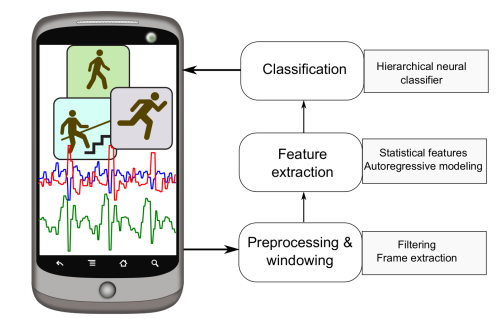
\includegraphics[width=0.9\textwidth]{Figs/DeteccionActividad1}
        \end{center}

\end{column}
\begin{column}{0.49\textwidth}
\begin{center}
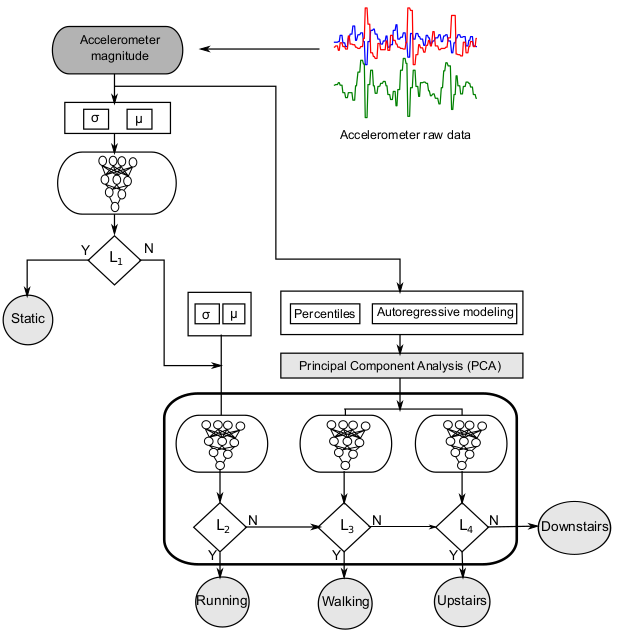
\includegraphics[width=0.7\textwidth]{Figs/DeteccionActividad5}
          \end{center}
\end{column}

\end{columns}
\end{block}
\end{frame}


\begin{frame}{\citetitle{MarcoNuno_CongArbIng_2015_02_00} (3)}
\begin{block}{Results (2)} 
\begin{columns}
\begin{column}{0.5\textwidth}
\begin{itemize}
\item The application power consumption profile and execution time of AR were obtained for several smartphones.
%\note[item]{\scriptsize In the bottom left we show a the comparison of three smartphones.}
\item The confusion matrix of the proposed AR system was obtained.  
\note[item]{\scriptsize The confusion matrix shows that the model discrimates well the different activities. 
}
%\note[item]{\scriptsize The bottom right table shows the timing in milliseconds for the processing steps on three devices; the time for AR model is enclosed in parentheses. }
\note[item]{\scriptsize On the bottom right screens of the proposed mobile app are shown. The application can operate in three different modes: data acquisition, offline processing for debugging purposes, and real-time activity continuous background monitoring. }

\end{itemize}
\begin{center}
%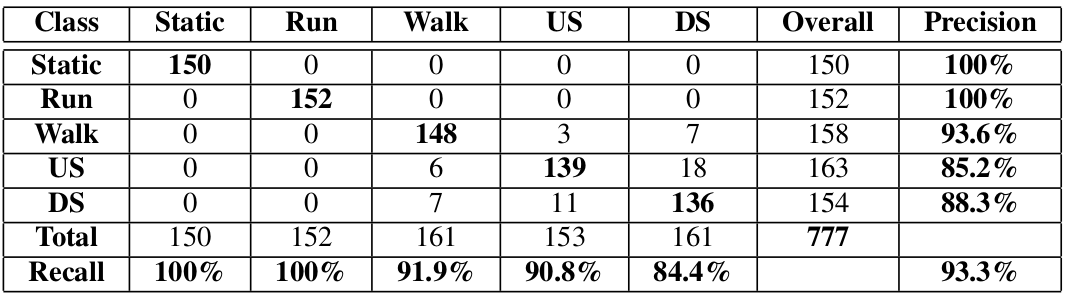
\includegraphics[width=0.9\textwidth]{Figs/DeteccionActividad6}
        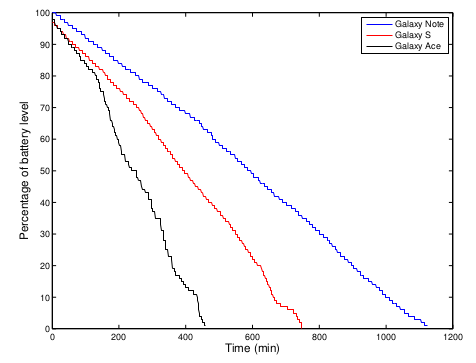
\includegraphics[width=0.5\textwidth]{Figs/DeteccionActividad4}
\end{center}
\end{column}
\begin{column}{0.5\textwidth}
    \begin{center}

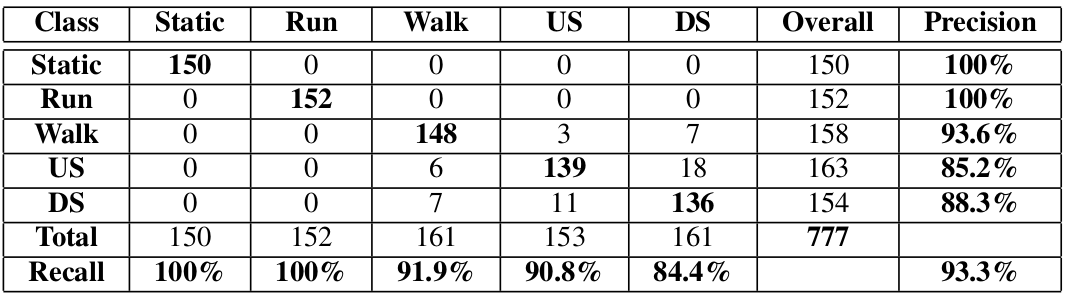
\includegraphics[width=0.8\textwidth]{Figs/DeteccionActividad6}
    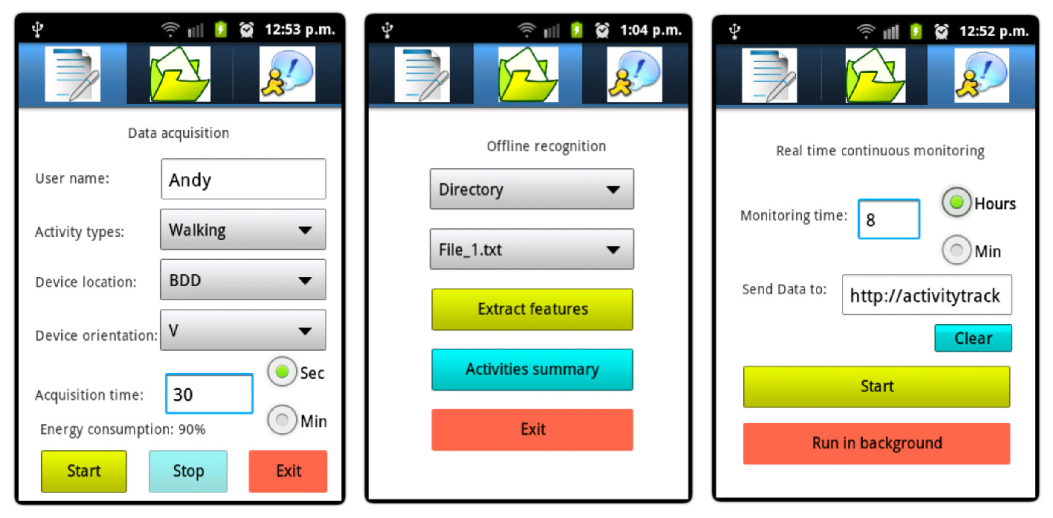
\includegraphics[width=0.95\textwidth]{Figs/DeteccionActividad7}
             %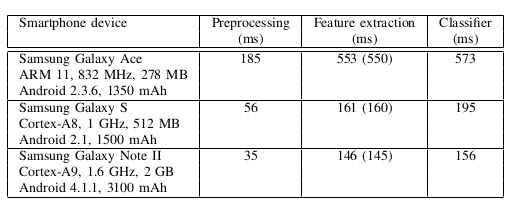
\includegraphics[width=0.6\textwidth]{Figs/DeteccionActividad3}
    \end{center}
\end{column}
\end{columns}
\end{block} 

% Conclusion ONE
\note[item]{\scriptsize A robust human activity recognition based on a single triaxial accelerometer has been proposed. It considers some typical locations where users carry out the smartphone without a firm attachment to the subject. A fully implementation on smartphones show near real-time performance and low power consumption thanks to the on-device lightweight processing.}

\end{frame}




